The  front-end  is  a software  tool  designed  to  provide  an easy  way  for
users to  model complicated  behaviours of photovoltaic  modules. The software
communicates with  the device via  a USB cable in  real time, which  means any
changes made  in the  tool have  an immediate effect  on the  generated output
voltage of the hardware device itself.

The front-end was built using the Qt framework\cite{ref:qt}, Qwt\cite{ref:qwt}
for 2D plots  and QwtPlot3D\cite{ref:qwtplot3d} for 3D plots,  and was written
in C++.  Qt was chosen because it  supports all major platforms and has a very
powerful set of  graphical components. Its Graphical User  Interface (GUI) can
be seen in  figure \ref{fig:front-end:screenshot}. On the left side  is a list
of  cells and  their  parameters. Cells can  be removed  or  added, and  their
individual  parameters  (open circuit  voltage,  short  circuit current,  dark
voltage  and  irradiation)  can  be  modified --  the  effects  of  which  are
immediate, as mentioned  above. A 2D plot shows what the  currently active I-V
characteristic curve looks like, along  with its corresponding power curve.  A
3D  plot  shows  the  behaviour  of  the  2D  power  curve  in  function  with
irradiation. In the  top right corner of  the GUI the actual  measured voltage
and current of the device is displayed.

\begin{figure}[th!]
    \centering
    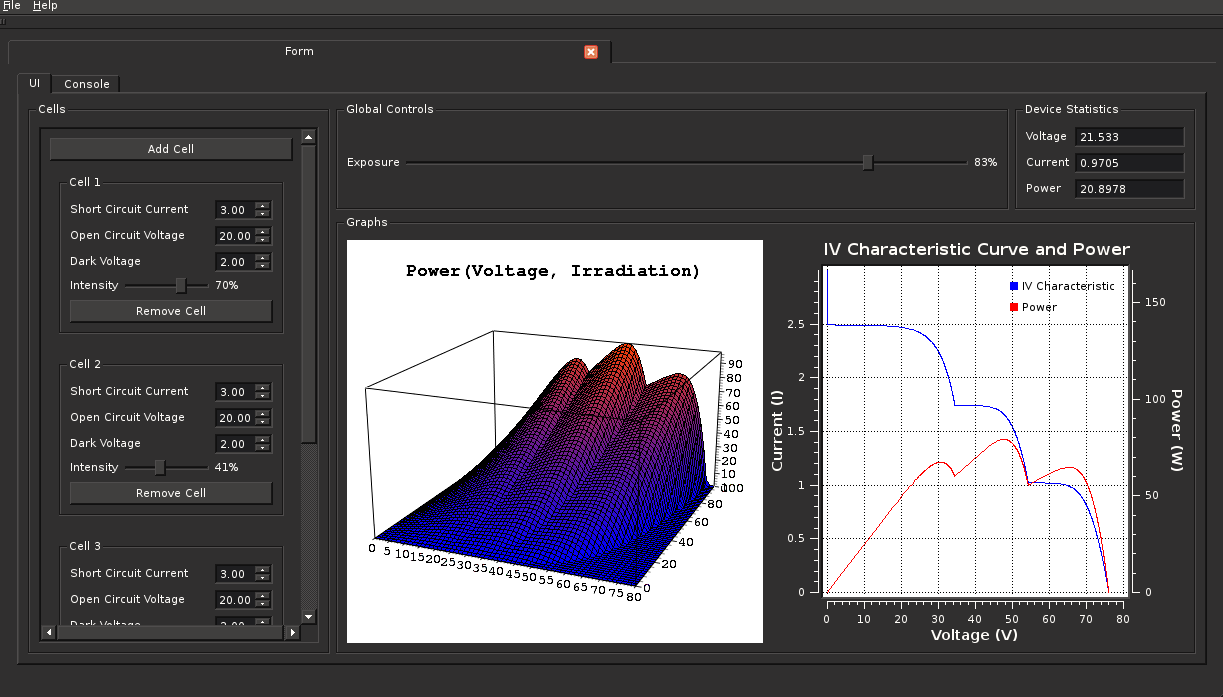
\includegraphics[width=.8\textwidth]{images/frontend/frontend.png}
    \caption{Screenshot of the front-end's Graphical User Interface (GUI)}
    \label{fig:front-end:screenshot}
\end{figure}

At this  point, the  front-end is  not yet  fully functional  as intended. The
graphical user  interface itself  is implemented  as planned,  but interfacing
with the  hardware lacks  yet a  few features. Partially,  this is  because we
could  not  test  all  its  functionality without  the  hardware  being  fully
operational. Another  reason  was  the   time  invested  into  diagnosing  the
issues related  to the buck converter  (section \ref{subsec:analysis_issue} on
pages  \pageref{subsec:analysis_issue}ff), which  needed to  be diverted  from
developing the front-end.

It is however in a solid proof-of-concept stage and ready to be finalised once
the device itself operates as intended.
